\section{MLPs training}\label{sec:mlptraining}

Script \texttt{mlptrain.m} performs the training of both networks. I use the
architecture selected in \secref{subsec:mlpbayesopt} for the ECG's mean
estimation network. For the ECG's standard deviation estimation network,
instead, I've selected a different architecture: the architecture chosen by
\code{bayesopt}, in fact, didn't gave me good results (\(R\) values between
\(0.35\) and \(0.5\)), probably due to a very lucky run during \code{bayesopt}.
So I've tested some other ``good'' architectures found by \code{bayesopt} and
I've found that the architecture of \code{bayesopt}'s epoch 74, with \(74\)
neurons in the first layer and \(29\) neurons in the second layer, gave me the
best results.

The new architecture (the one actually used) for the ECG's standard deviation
estimation network is shown in \figref{fig:mlpstdnewarch}.

\begin{figure}[htbp]
	\centering
	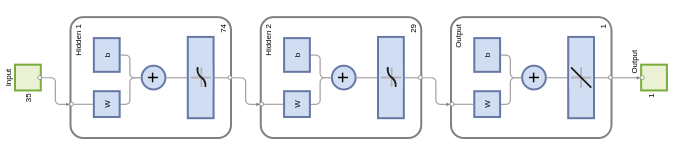
\includegraphics[width=\textwidth]{mlpstdnewarch}
	\caption{A new (and better) architecture for the ECG's standard
	deviation estimation network.}\label{fig:mlpstdnewarch}
\end{figure}

\begin{figure}[htbp]
	\centering
	\begin{subfigure}{\textwidth}
		\centering
		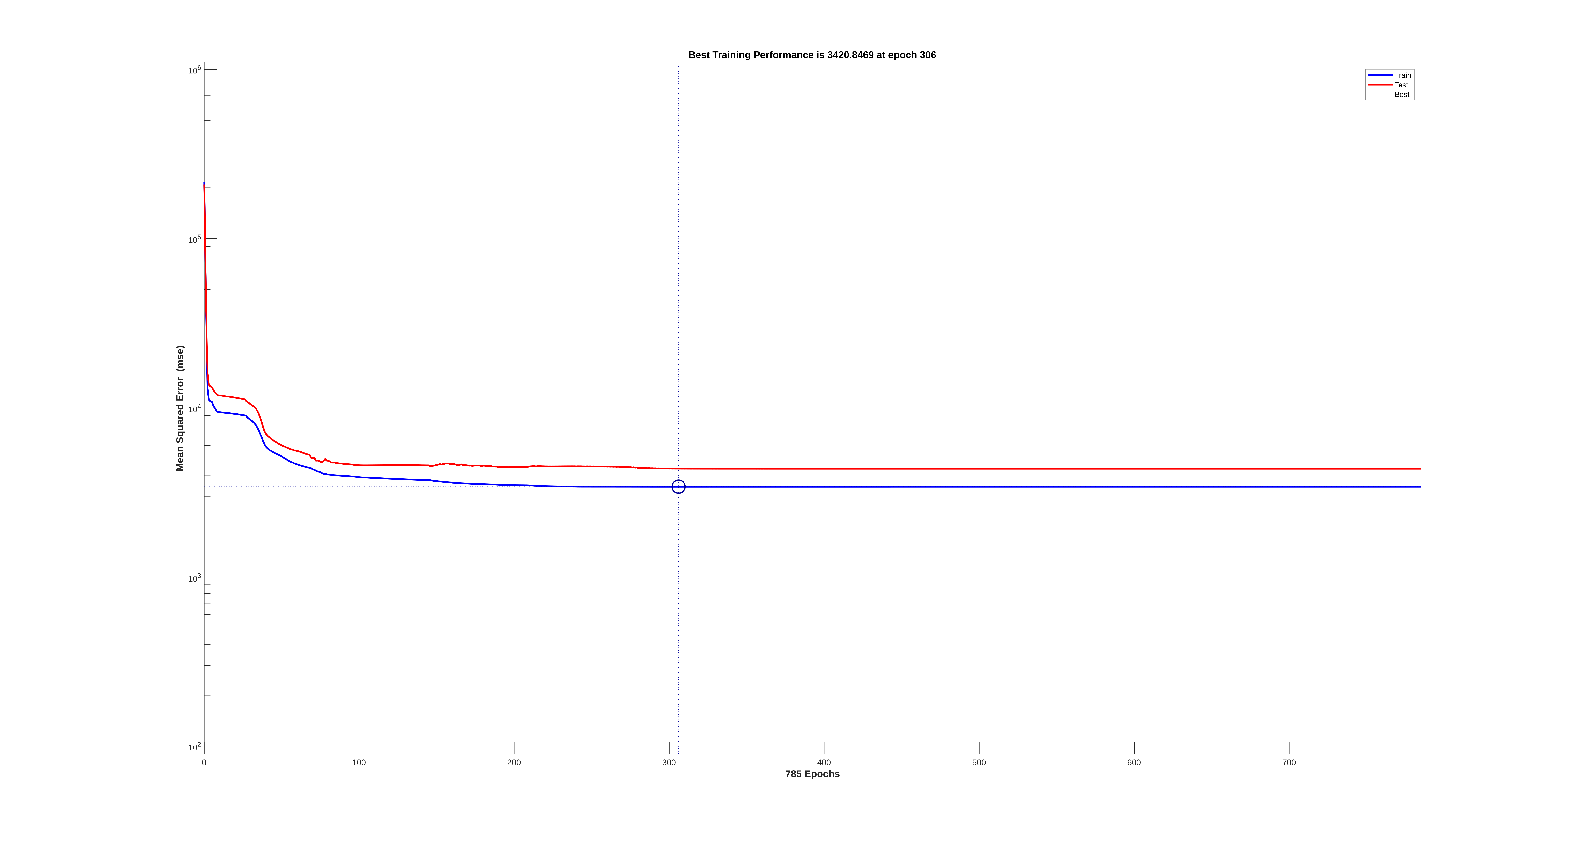
\includegraphics[width=\textwidth, trim=2.95cm 1.1cm 2cm 0.8cm,
		clip]{mlpmeantrainperformance}
		\caption{Training performance plot for the ECG's mean
		estimation network.}\label{fig:mlpmeantrainperformance}
	\end{subfigure}
	\begin{subfigure}{\textwidth}
		\centering
		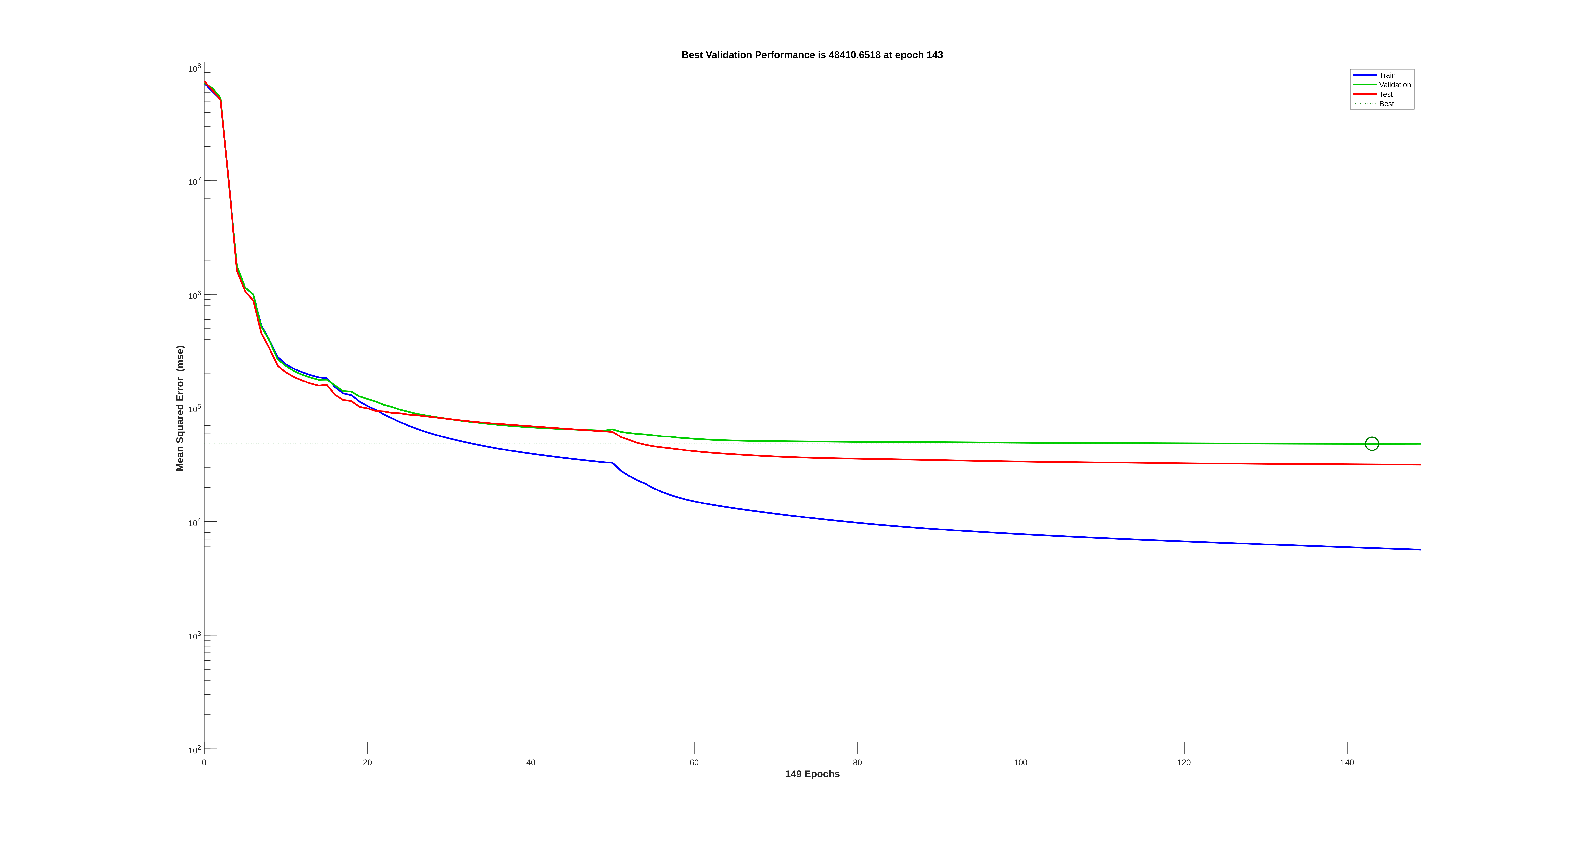
\includegraphics[width=\textwidth, trim=2.95cm 1.1cm 2cm 0.8cm,
		clip]{mlpstdtrainperformance}
		\caption{Training performance plot for the ECG's standard
		deviation estimation network.}\label{fig:mlpstdtrainperformance}
	\end{subfigure}
	\caption{Training performance plots for the two
	networks.}\label{fig:mlptrainperformance}
\end{figure}

The ECG's mean estimation network performances are quite good, as shown in
\vfigref{fig:mlpmeanregression}: we have \(R = 0.85045\) for the test set and
\(R = 0.85761\) for the entire dataset.

\begin{figure}[htbp]
	\centering
	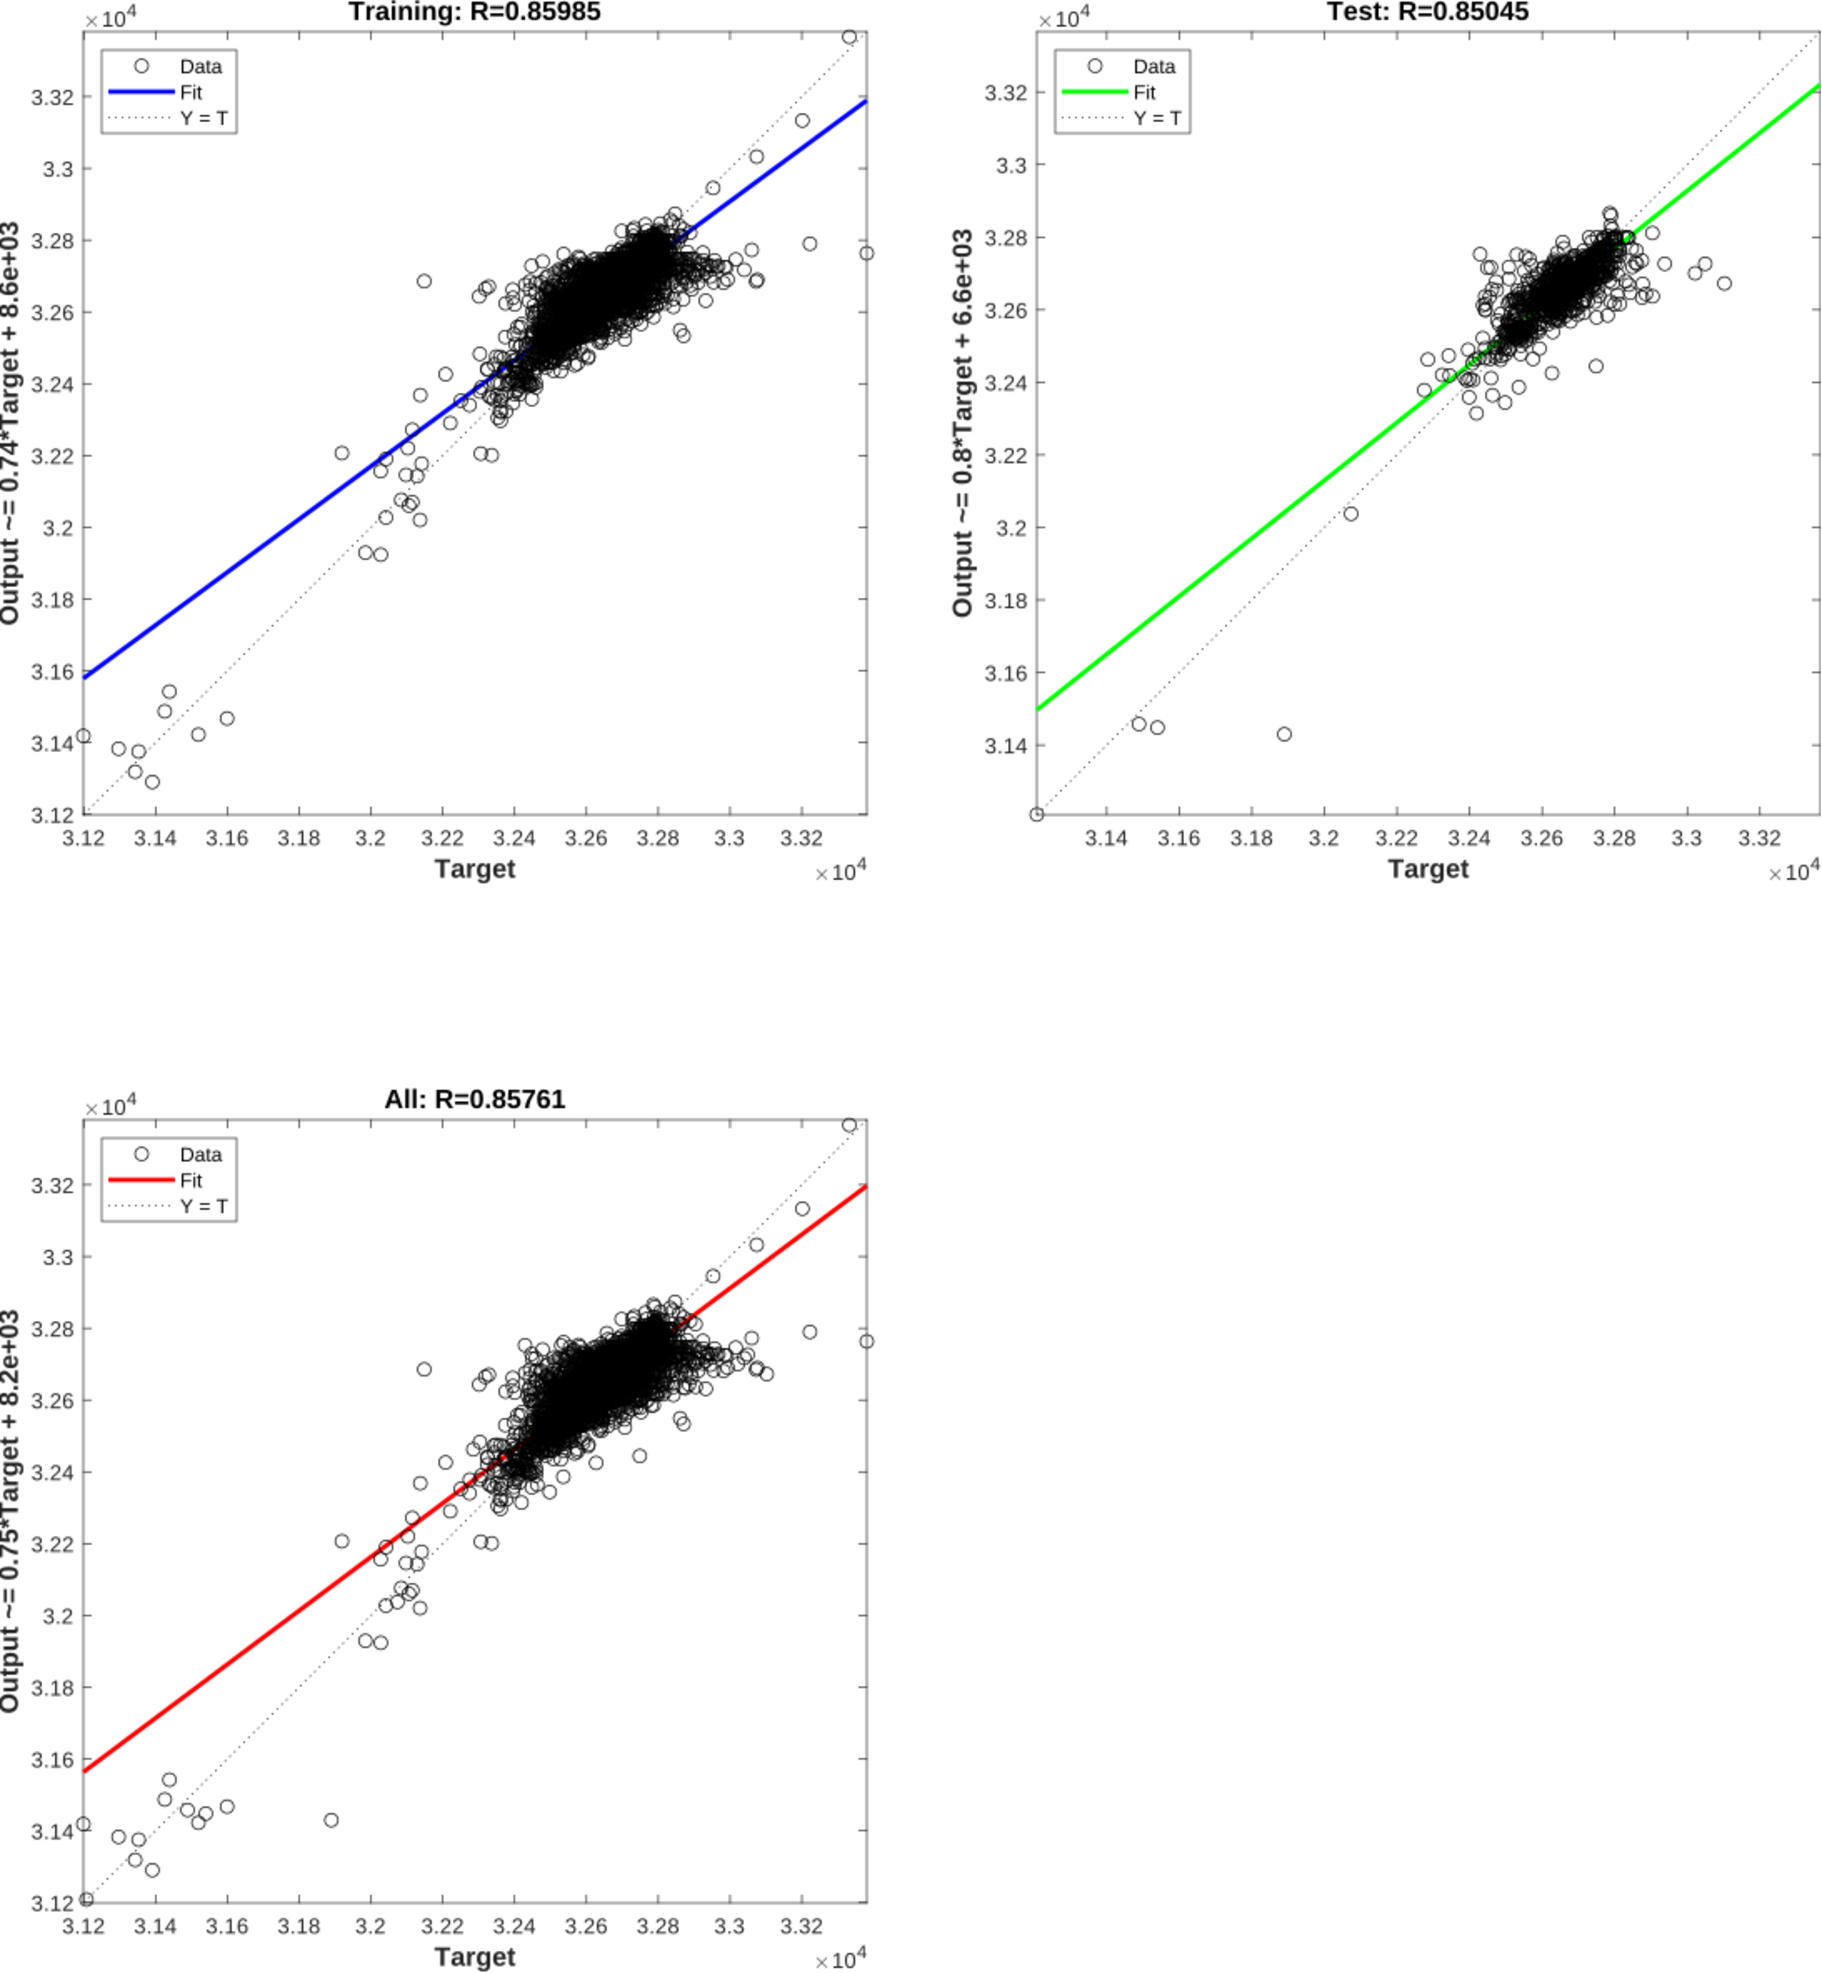
\includegraphics[width=\textwidth]{mlpmeanregression}
	\caption{The regression plot for the ECG's mean estimation network
	shows good results.}\label{fig:mlpmeanregression}
\end{figure}

\vfigref{fig:mlpstdregression} shows the regression plot for the ECG's standard
deviation estimation network. The network performarce are not so good, with a
coefficient \(R = 0.58968\) for the test set and \(R = 0.61487\) for the entire
dataset. This latter network will be the subject of \chref{ch:cnn}.

\begin{figure}[htbp]
	\centering
	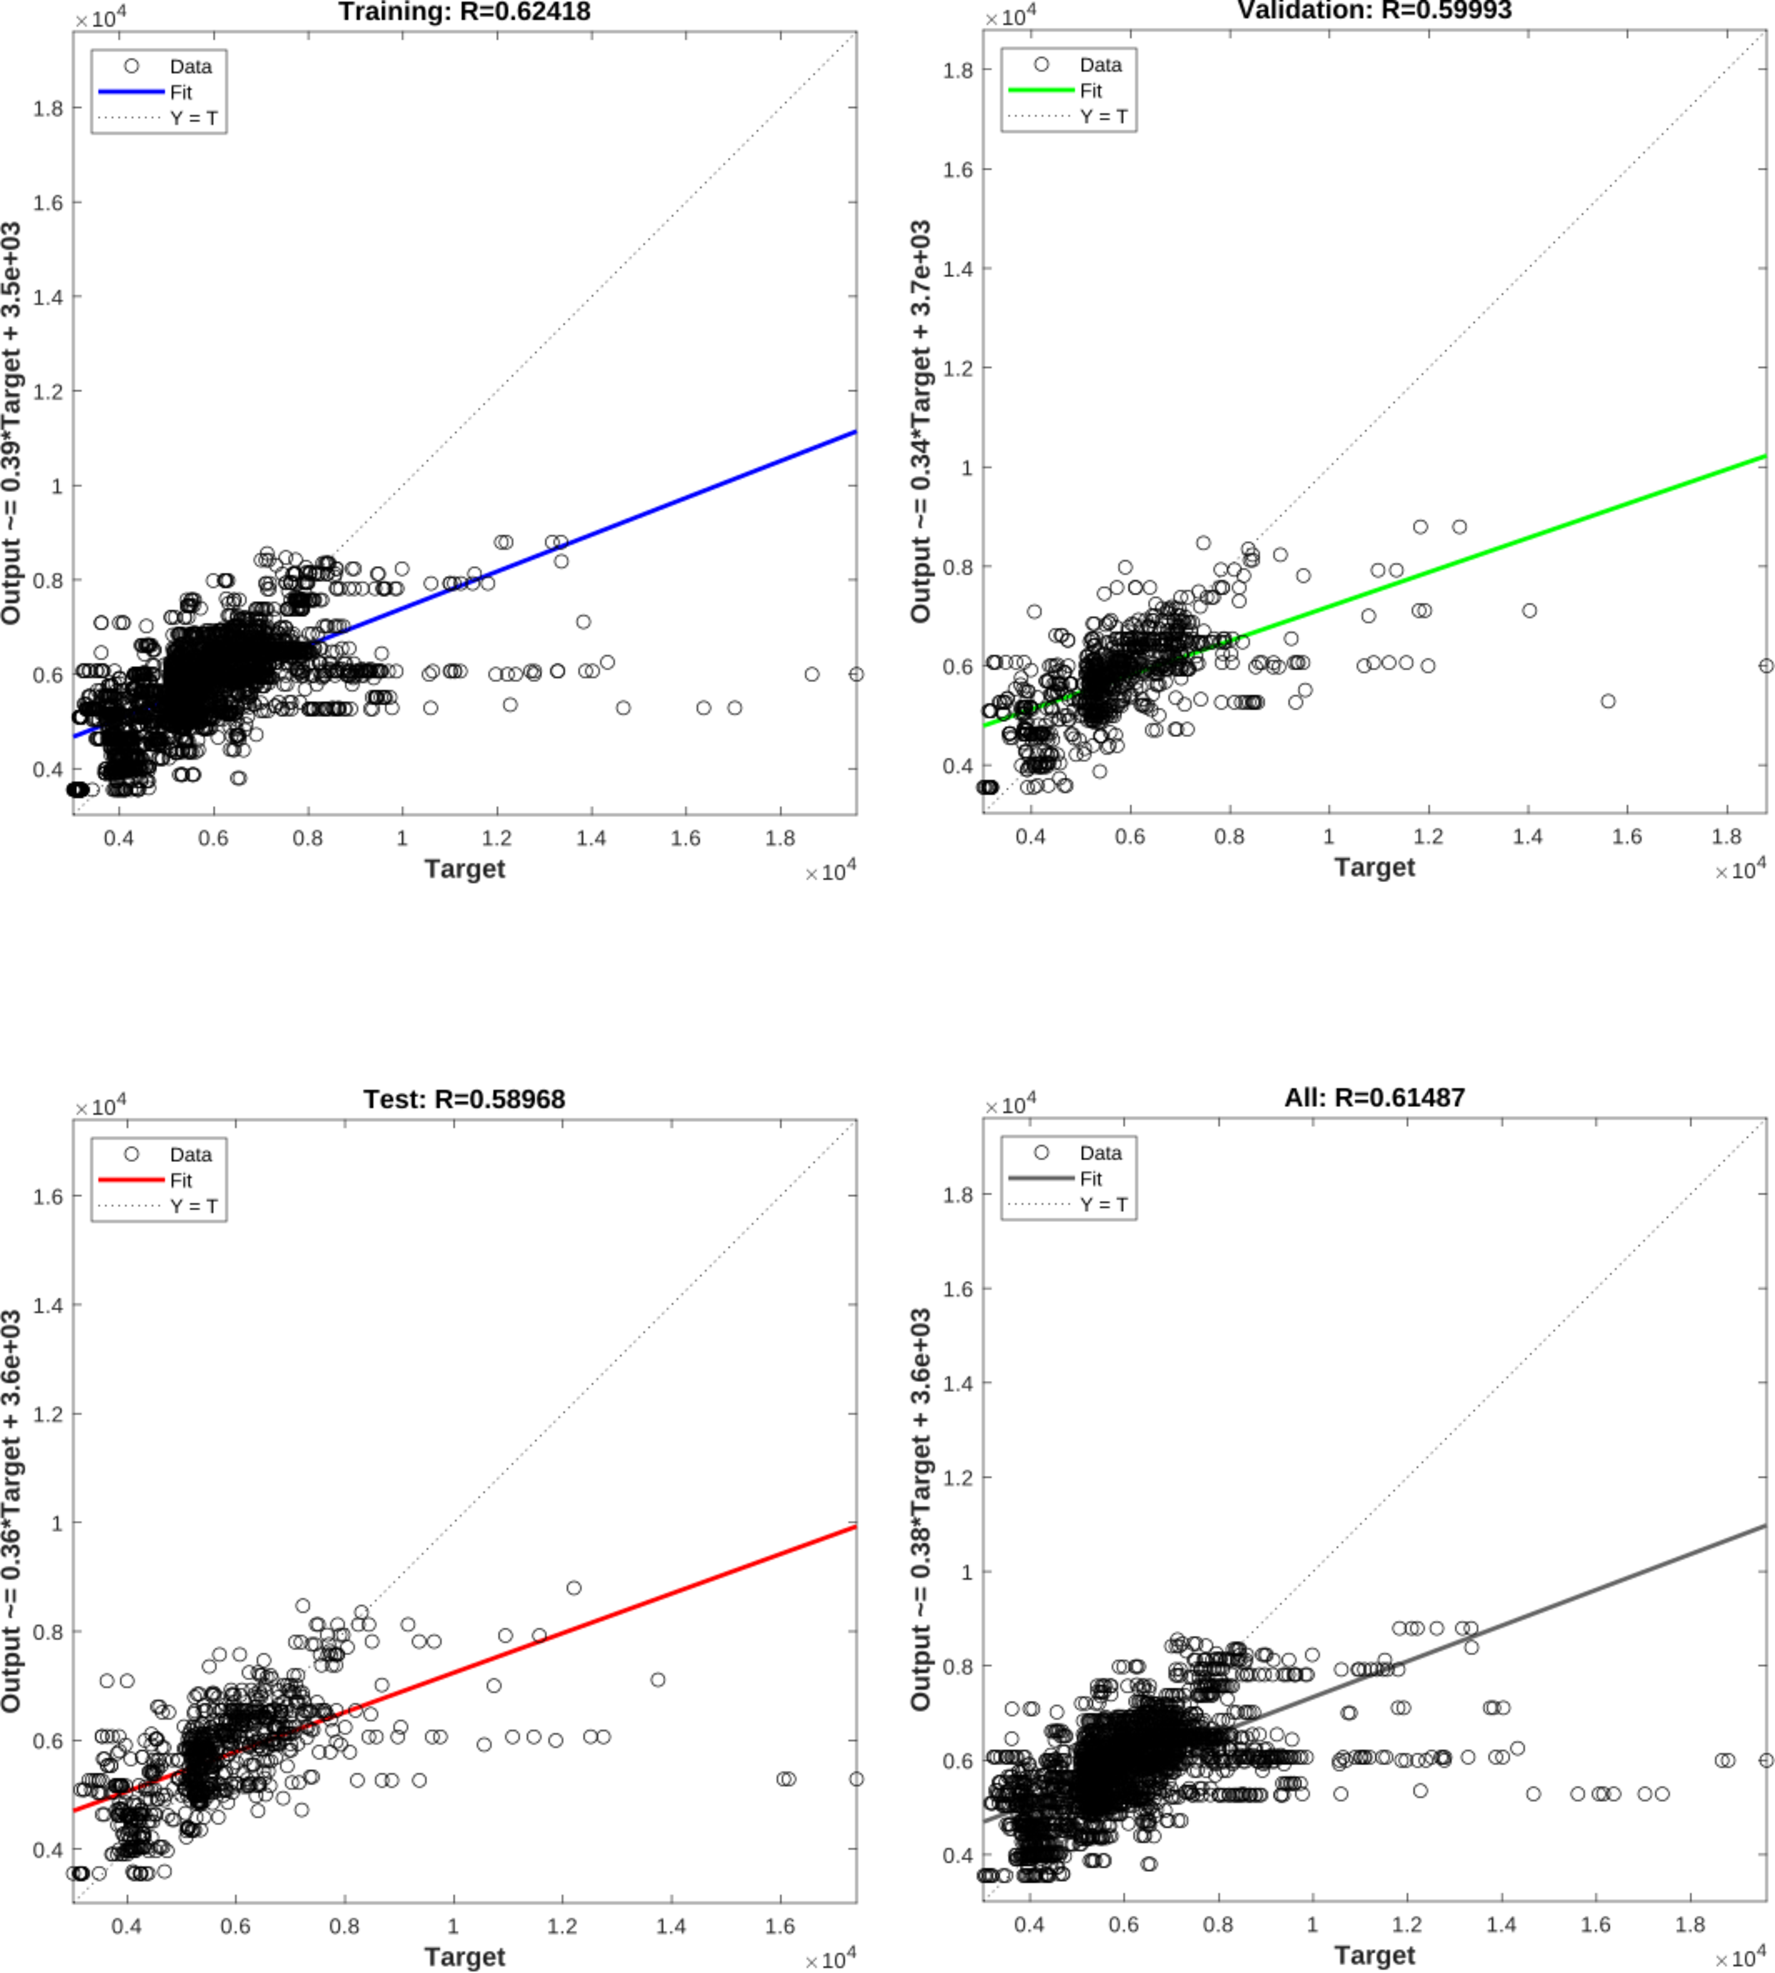
\includegraphics[width=\textwidth]{mlpstdregression}
	\caption{The regression plot for the ECG's standard deviation
	estimation network shows quite bad
	results.}\label{fig:mlpstdregression}
\end{figure}

\begin{figure}[htbp]
	\centering
	\begin{subfigure}{\textwidth}
		\centering
		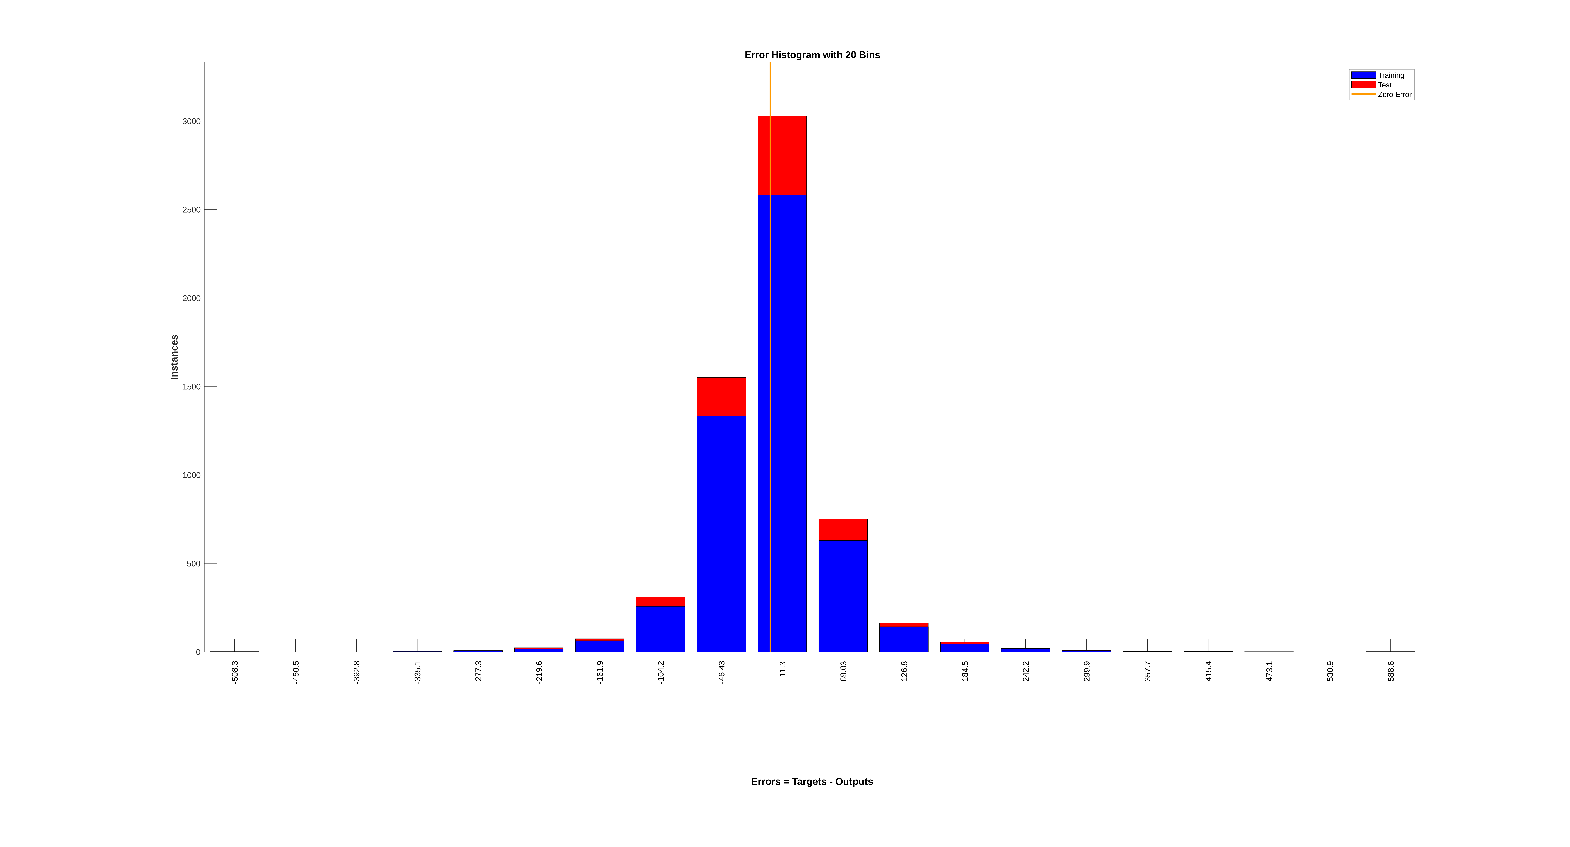
\includegraphics[width=\textwidth, trim=2.9cm 1cm 2cm 0.8cm,
		clip]{mlpmeanerrorhist}
		\caption{Error histogram for the ECG's mean estimation
		network.}\label{fig:mlpmeanerrorhist}
	\end{subfigure}
	\begin{subfigure}{\textwidth}
		\centering
		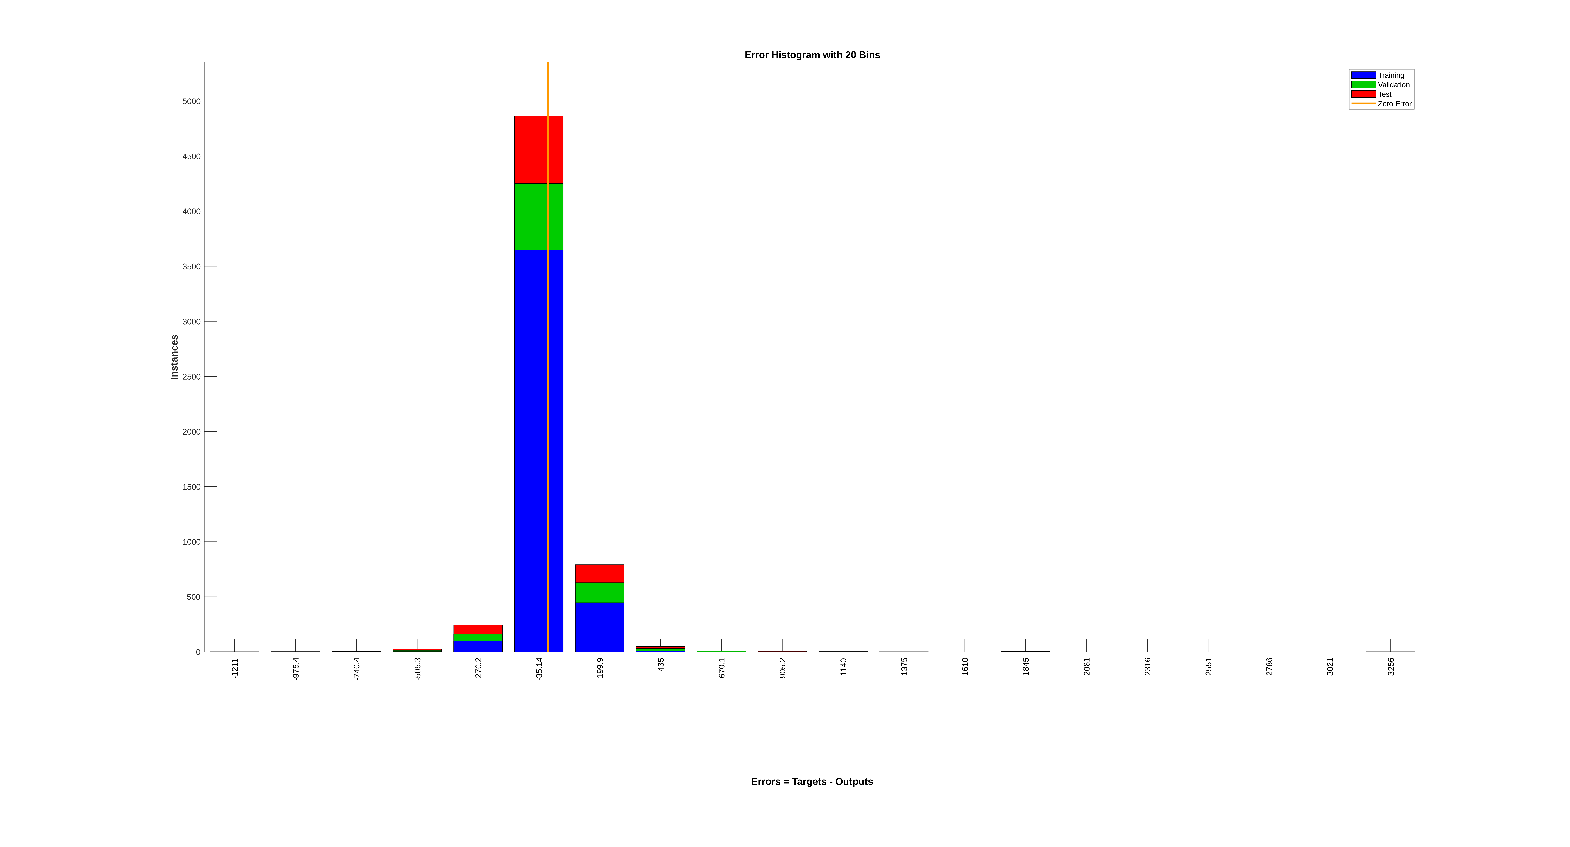
\includegraphics[width=\textwidth, trim=2.9cm 1cm 2cm 0.8cm,
		clip]{mlpstderrorhist}
		\caption{Error histogram for the ECG's standard deviation
		estimation network.}\label{fig:mlpstderrorhist}
	\end{subfigure}
	\caption{Error histograms for the two
	networks.}\label{fig:mlperrorhists}
\end{figure}
